%sudo apt install libboost-all-dev
%sudo apt install libcurlpp-dev
%sudo apt install libcurl4-openssl-dev
%sudo apt install libssl-dev
%sudo apt install uuid-dev
%https://github.com/beniz/deepdetect/issues/126
%https://github.com/Azure/azure-iot-sdk-c/blob/master/doc/devbox_setup.md
%https://github.com/Azure/azure-iot-sdk-c/blob/master/doc/ubuntu_apt-get_sample_setup.md
%https://www.rti.com/gettingstarted/installlinux_secure
%https://unix.stackexchange.com/questions/389156/how-to-fix-held-broken-packages/389170

\LoadClass[a4paper]{article}
\documentclass{article}

\usepackage{listings}
\lstset{
basicstyle=\ttfamily,
columns=flexible,
breaklines=true
}
\usepackage{color}

\definecolor{mygray}{rgb}{0.4,0.4,0.4}
\definecolor{mygreen}{rgb}{0,0.0,0.6}
\definecolor{myorange}{rgb}{1.0,0.4,0}

\lstset{
commentstyle=\color{mygray},
frame=none,
numbersep=5pt,
numberstyle=\tiny\color{mygray},
keywordstyle=\color{mygreen},
showspaces=false,
showstringspaces=false,
stringstyle=\color{myorange},
tabsize=2
}

\usepackage{verbatim}

\usepackage[hidelinks]{hyperref}
\hypersetup{
	colorlinks=true,
    pdfborder={0 0 0},
    urlcolor     = blue, %Colour for external hyperlinks
    linkcolor    = blue, %Colour of internal links
    citecolor   = red %Colour of citations
}

\usepackage{titlesec}
\newcommand{\sectionbreak}{\clearpage}

\usepackage{graphicx}

\author{Janos Benjamin Antal\\\href{mailto:antal.janos.benjamin@gmail.com}{antal.janos.benjamin@gmail.com}}
\title{CPS Humidity Homework}
\begin{document}
\maketitle
\section{Homework description}
The task in this homework is to design and develop one subsystem of an imaginary "smart" university control system. The subsystem's goal is to help keep the humidity of a classroom in the desired range. The subsystem has to interferes with the control system based on information gathered from the sensors in a classroom and some online services. The subsystem must contains at least a local and an online module communicating each other. Furthermore, the subsystem should grant a minimal level of assurance The subsystem should store the gathered information and controlling decision in the cloud for further alanysis.
\begin{itemize}
\item \textbf{Sensors}: a humidity sensor inside the classroom
\item \textbf{Interferer}: a LED on the teacher's desk to indicate the opening/closing of the window: the window should be opened when the LED turns on, and should be closed when the LED turns off
\item \textbf{Services}: a weather forecast and a schedule information provider service
\item \textbf{Assurance}: in case of the weather is too hot or the air too polluted the subsystem shouldn't indicate the opening of window. When the classroom is not scheduled, the maximum of humidity should be bigger than it's scheduled.
\end{itemize}
\section{Requirements} The requirements above are really high level requirements, and in a real situation they should be refined to low level specifications. The requirements are specified as sentences and also most of them as Gherkin test cases: \\
\begin{itemize}

\item \textit{Turn on the only when the outer conditions are right and the humidity reach the upper bound:}
\begin{verbatim}
Given the system with right humidity value in the classroom
And the LED is turned on
And the temperature is not too high
And the air pollution level is not too high
When the humidity reaches the upper bound
Then after the next refresh the LED turns on
\end{verbatim}
\item \textit{Turn off the LED when humidity reaches the lower bound:}
\begin{verbatim}
Given the system with humidity value above the upper boundary
And the LED is turned on
And the temperature is not too high
And the air pollution level is not too high
When the humidity reaches the lower bound
Then after the next refresh the LED turns off
\end{verbatim}
\item \textit{Turn off the LED when the temperature becomes too high:}
\begin{verbatim}
Given the system with humidity value above the upper boundary
And the LED is turned on
And the temperature is not too high
And the air pollution level is not too high
When the temperature becomes too high
Then after the next refresh the LED turns off
\end{verbatim}
\item \textit{Turn off the LED when the air pollution becomes too high:}
\begin{verbatim}
Given the system with humidity value above the upper boundary
And the LED is turned on
And the temperature is not too high
And the air pollution level is not too high
When the air pollution becomes too high
Then after the next refresh the LED turns off
\end{verbatim}
\item \textit{Never turn on the LED when the air pollution level is too high:}
\begin{verbatim}
Given the system with right humidity value in the classroom
And the LED is turned off
And the air pollution is too high
When the humidity raise above the upper boundary
Then after the next refresh the LED is still turned off
\end{verbatim}
\item \textit{Never turn on the LED when the outer temperature is too high:}
\begin{verbatim}
Given the system with right humidity value in the classroom
And the LED is turned off
And the temperature is too high
When the humidity raise above the upper boundary
Then after the next refresh the LED is still turned off
\end{verbatim}
\item \textit{The subsystem must communicate with sensors placed in the classroom:}
\begin{verbatim}
Given the system with three fully operational sensor
And the system can get humidity value from each sensor
\end{verbatim}
\textit{The subsystem can turn on the LED:}
\begin{verbatim}
Given the system with right humidity value in the classroom
And the LED is turned off
When the humidity reaches the upper bound
Then after the next refresh the LED turns on
\end{verbatim}
\item \textit{Use encryption and certification in communication with cloud:}
\begin{verbatim}
Given the system
When the system sends status information to the cloud
Then the cloud server proofs that its the right server
And the message is encrypted
\end{verbatim}
\item \textit{After the decision made, the actual status must be saved to the cloud.}\\
\item \textit{Parameters (humidity boundaries, maximum air pollution level and maximum temperature) can be configurated remotely.}
\item \textit{The subsystem must communicate with weather forecast system.}
\item \textit{The subsystem must communicate with schedule information provider.}
\item \textit{The subsystem must communicate with external systems by "best practice" protocols.}
\item \textit{The subsystem must take into consideration the unavailability of external data sources when deciding on turning on/off the LED.}
\end{itemize}

\section{System architecture}
\begin{figure}[!htb]
  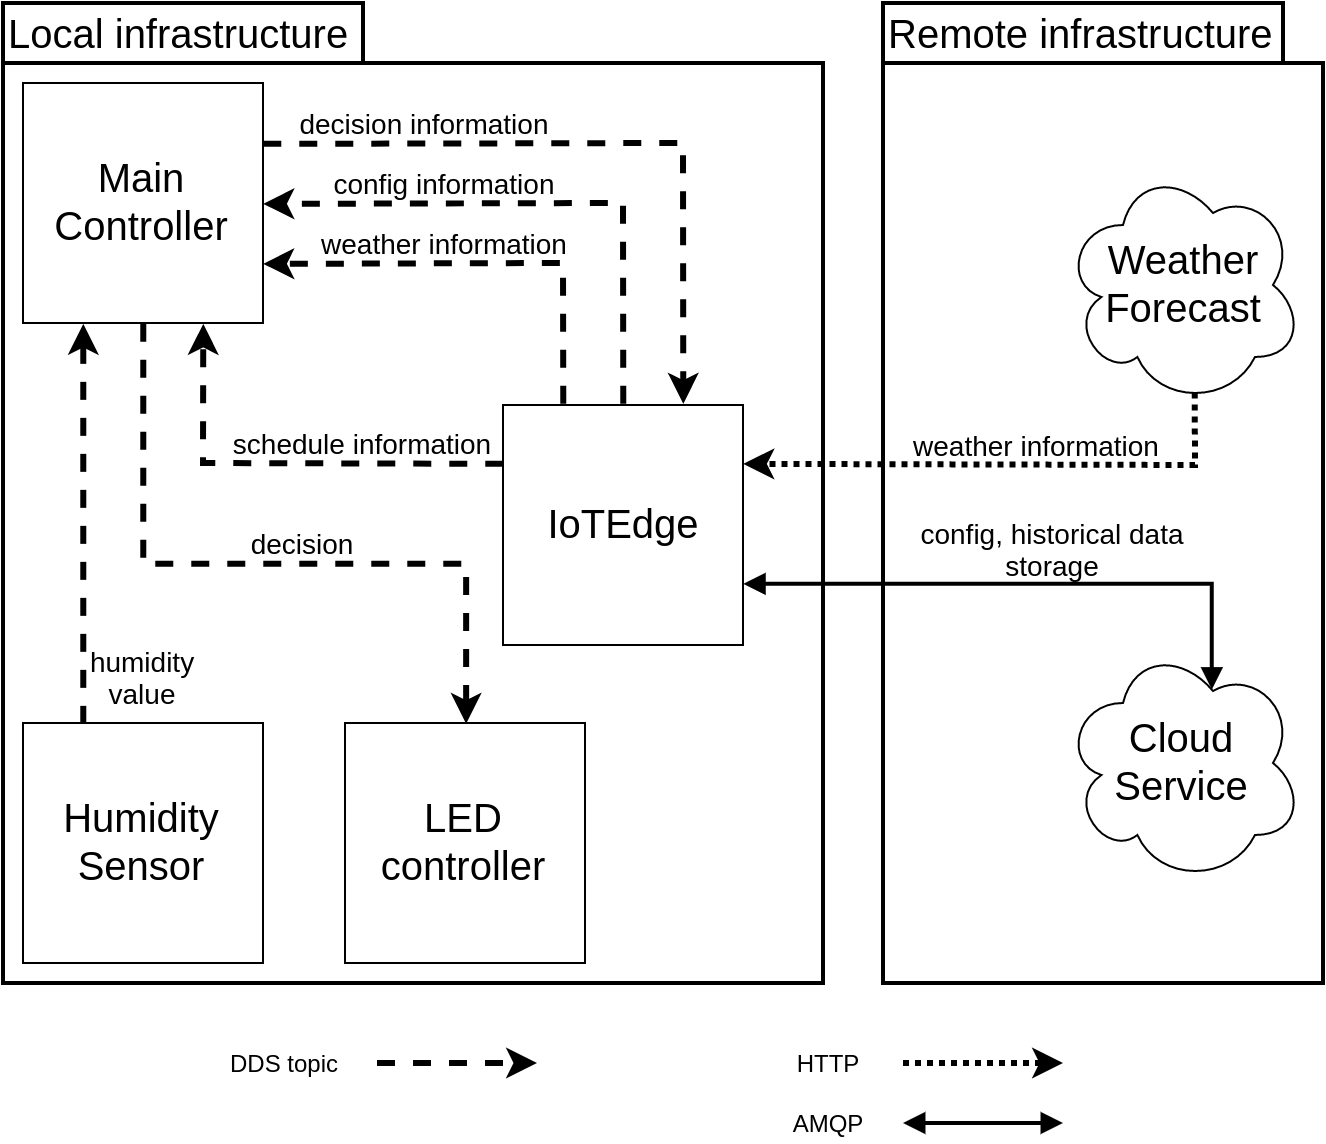
\includegraphics[width=\linewidth]{imgs/system_architecture.png}
  \caption{The system semantic architecture}
  \label{fig:system_architecture}
\end{figure}
In the first approach, we split the system into two disjoint part: the local and remote infrastructure. As the figure \ref{fig:system_architecture} shows, the local infrastructure contains the IoTEdge, controller and humidity sensor modules. They only communicate over DDS topics. The reason behind this is that in this way the infrastructure is easily can be expanded, because new modules also can subscribe to DDS topics and use the information sended over them. The local infrastructure contains four modules:
\begin{itemize}
\item \textbf{IoTEdge}: The IoTEdge module is responsible for comunication with the remote infrastructure, which consists the cloud service and the weather forecast system. It also communicate with the Main Controller: edge send the weather, schedule and config information to it and receives the information that serves as the basis of decision making.
\item \textbf{Main Controller}: The main controller receives the required information and sensor values and also make decisions based on the collected data. It also sends the decision input and output to the IoTEdge in order to store them in the cloud.
\item \textbf{Humidity Sensor}: The sensor goals is to periodically measure and publish the humidity value of the classroom.
\item \textbf{LED Controller}: As its name says it has to turn on/off the LED according to the main controller's decision. It's logically separated from the main controller.
\end{itemize}
It has to be noticed that the local infrastructure is only a semantic architecture, so it has to mapped to physical device or devices. The four modules can be hosted on a single device or four separated devices. The figure TODOOO shows a possible mapping to physical devices:
\begin{figure}[!htb]
\centering
  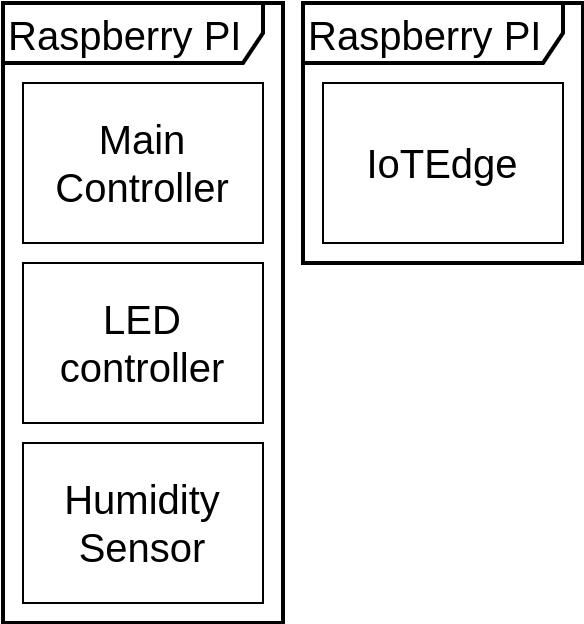
\includegraphics[width=150px]{imgs/phisical_mapping.png}
  \caption{A possible mapping to physical devices}
  \label{fig:phisical_mapping}
\end{figure}
\section{Implementation}
The implemented modules are the following:
\begin{itemize}
\item IoTEdge
\item Controller
\item Humidity Publisher
\end{itemize}
The publisher module exists only for mocking the real humidity sensor, so this documentation doesn't contains its details. There is no implementation of LED Controller, because this isn't in the focus of this homework.
\subsection{IoTEdge}
\begin{figure}[!htb]
  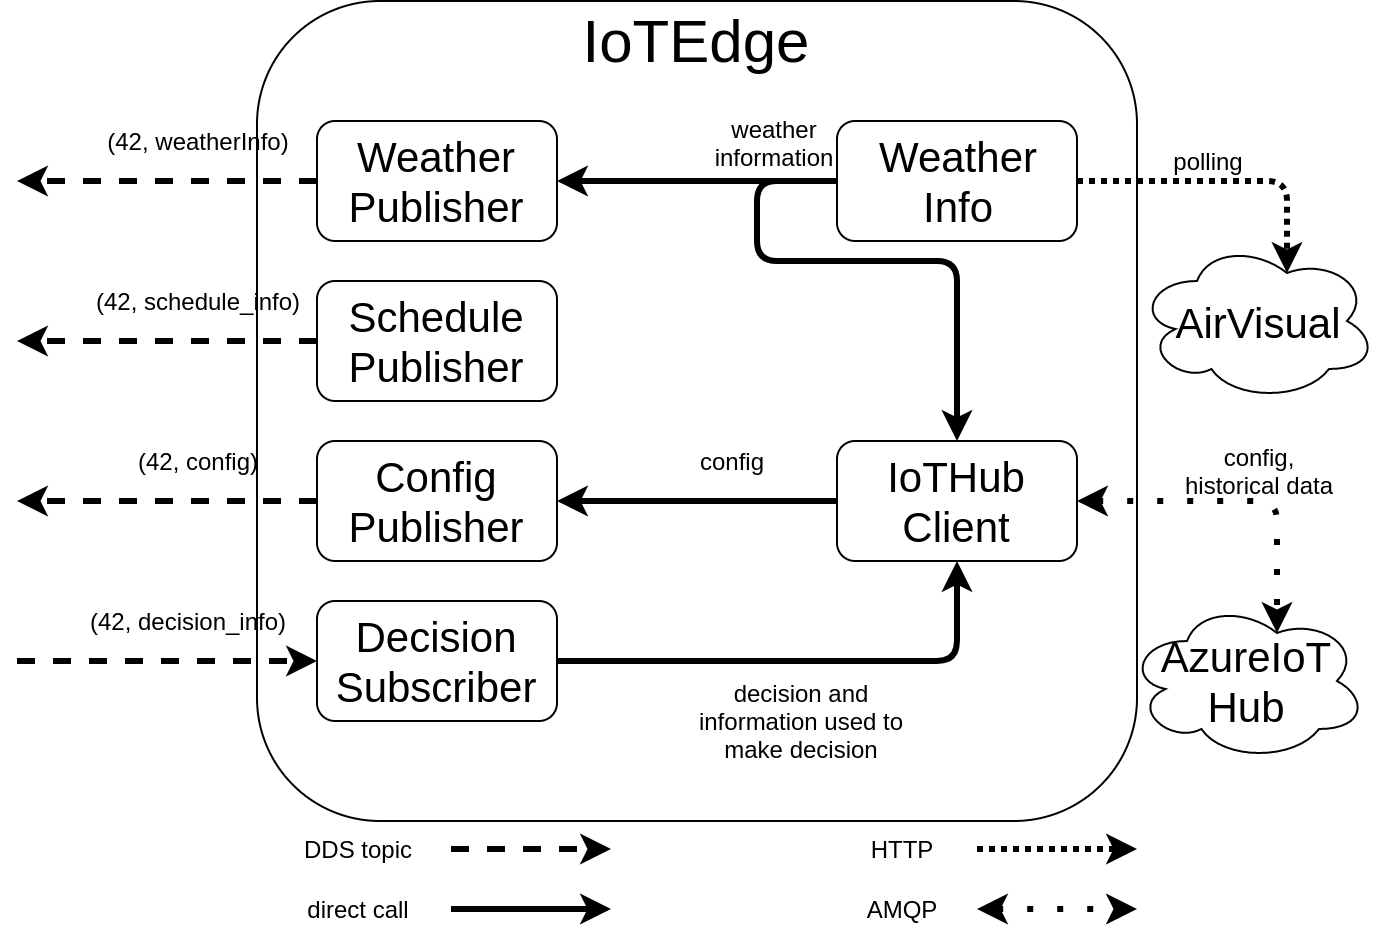
\includegraphics[width=\linewidth]{imgs/edge.png}
  \caption{Inner architecture of IoT Edge}
  \label{fig:arc_edge}
\end{figure}

As the figure \ref{fig:arc_edge} shows, the IoTEdge translates the messages received from the cloud and the weather forecast API to DDS messages and vica versa. The DDS Interface Description Language exactly describe the contents of the used DDS messages:
\begin{verbatim}
struct Config {
    double maxTemperature;
    unsigned long maxPollution;
    unsigned long minHumidity;
    unsigned long maxHumidity;
};

struct Schedule {
    boolean scheduled;
    unsigned long until;
    unsigned long sentTS;
};

struct UvegHaz{
    string ID; //@key
    double Value;
    long TimeStamp;
};

struct Weather {
    double  temperature;
    unsigned long tempTS;
    unsigned long pollution;
    unsigned long pollTS;
};

enum Decision { CLOSE, OPEN };

struct DecisionInfo {
    unsigned long decisionTS;
    Decision decision;
    Config config;
    Weather lastWeather;
    Schedule lastSchedule;
    UvegHaz lastHumidity;
};
\end{verbatim}

The most complex part of the IoTEdge module is the IoTHub Client. It is responsible for translating and communicating between the IoTEdge and AzureIoT Hub. It sends the received sensor, weather and decision data to the cloud, and also receives config message from it. A config message contains the maximum outside temperature, the maximum outside pollution and the desired minimum and maximum temperature in the classroom. For example:
\begin{verbatim}
{
    "maximumTemperature" : 50,
    "maximumPollution" : 55,
    "minimumHumidity" : 42,
    "maximumHumidity" : 46
}
\end{verbatim}
\begin{itemize}
\item maximumTemperature: a temperature value in Celsius. If the outside temperature reaches this limit, the controller logic mustn't decide to open the window.
\item maximumPollution:  a pollution value in Air Quality Index. If the outside pollution reaches this limit, the controller logic mustn't decide to open the window.
\item minimumHumidity, maximumHumidity: the desired range of humidity expressed as relative humidity. The goal of the system it to keep humidity within this range.
\end{itemize}
\subsubsection{IoTHub Client}

The IoTHub Client is a reusable part of the implementation. It's public interface are really simple:

\begin{lstlisting}[language=C++]{Name=iothub_client}
class IoTHubClient final {
public:

    IoTHubClient(const std::string &connectionString,
                 std::function<void(const rapidjson::Document &)> receivedMessageConsumer, 
                 bool trace = false,
                 uint32_t keepAlive = 240);

    ~IoTHubClient();

    void start();

    void stop();

    void sendMessage(const rapidjson::Document &message);
};
\end{lstlisting}

The implementation is based on an official Azure IoT C SDK \href{https://github.com/Azure/azure-iot-sdk-c/blob/master/iothub_client/samples/iothub_client_sample_amqp/iothub_client_sample_amqp.c}{example}. Usage of the module also really simple. The constructor takes an Azure IoT Hub decive connection string, a message consumer function and two other parameters. More information about the last two parameters can be found in the referenced example. To start receiving/sending messages with an existing instance of IoTHubClient, the \verb+start()+ function has to be called. After the calling, the instance starts to receive messages from IoT Hub and also sends messages to it when \verb+sendMessage(msg)+ is called.

\subsubsection{Abstract DDS classes}

All of the \verb+XXXPublisher+ and the \verb+XXXSubscriber+ in this project is derived from \verb+AbstractPublisher+ and \verb+AbstractSubscriber+. They are generic template classes in order to make easy to create DDS publishers and subscribers. The interface of \verb+AbstractPublisher+ is the following:
\begin{lstlisting}[language=C++]{Name=publisher}
template<typename DataT>
class AbstractPublisher {
public:
    AbstractPublisher(int domain_id,
                      const std::string &topic_name);

    virtual ~AbstractPublisher();

    void publishData(const DataT &data);
};
\end{lstlisting}
The \verb+DataT+ template parameter should be DDS generated message's type. The \verb+publishData(data)+ function can be used to send a message to the given topic.

The \verb+AbstractSubscriber+'s interface is very similar:
\begin{lstlisting}[language=C++]{Name=subscriber}
template<typename DataT>
class AbstractSubscriber : public dds::sub::NoOpDataReaderListener<DataT> {
public:

    AbstractSubscriber(int domain_id, 
                       const std::string &topic_name, 
                       int pollSeconds);

    virtual ~AbstractSubscriber();

    void on_data_available(dds::sub::DataReader<DataT> &reader) override ;

    void startReceiving(std::function<void(const DataT &data)> consumerFunction);

    void stopReceiving();
};
\end{lstlisting}

The \verb+on_data_available(dds::sub::DataReader<DataT> &reader)+ inherited from the base class, and shouldn't be called by the user. To start receiving messages the \verb+startReceiving(consumerFunction)+ function has to be called. After that, the subscriber will call the \verb+consumberFunction+ when a new message arrives.

\subsection{Controller}
The Controller receives the DDS messages with the required informations (scheduling, weather information, measured sensor values and configuration messsages), and makes decision based on them. Figure \ref{fig:decision_logic} shows the exact process of decision making. Decision making runs periodically in each 5 minutes, and decision is also made on receiving every input messages. It's important to make decision independently to message receiving, because the last known informations can be outdated. In case of any information is outdated, the decision output must be \verb+CLOSED+ in order to avoid opened window under not safe circumstances.
\begin{figure}[!htb]
\centering
  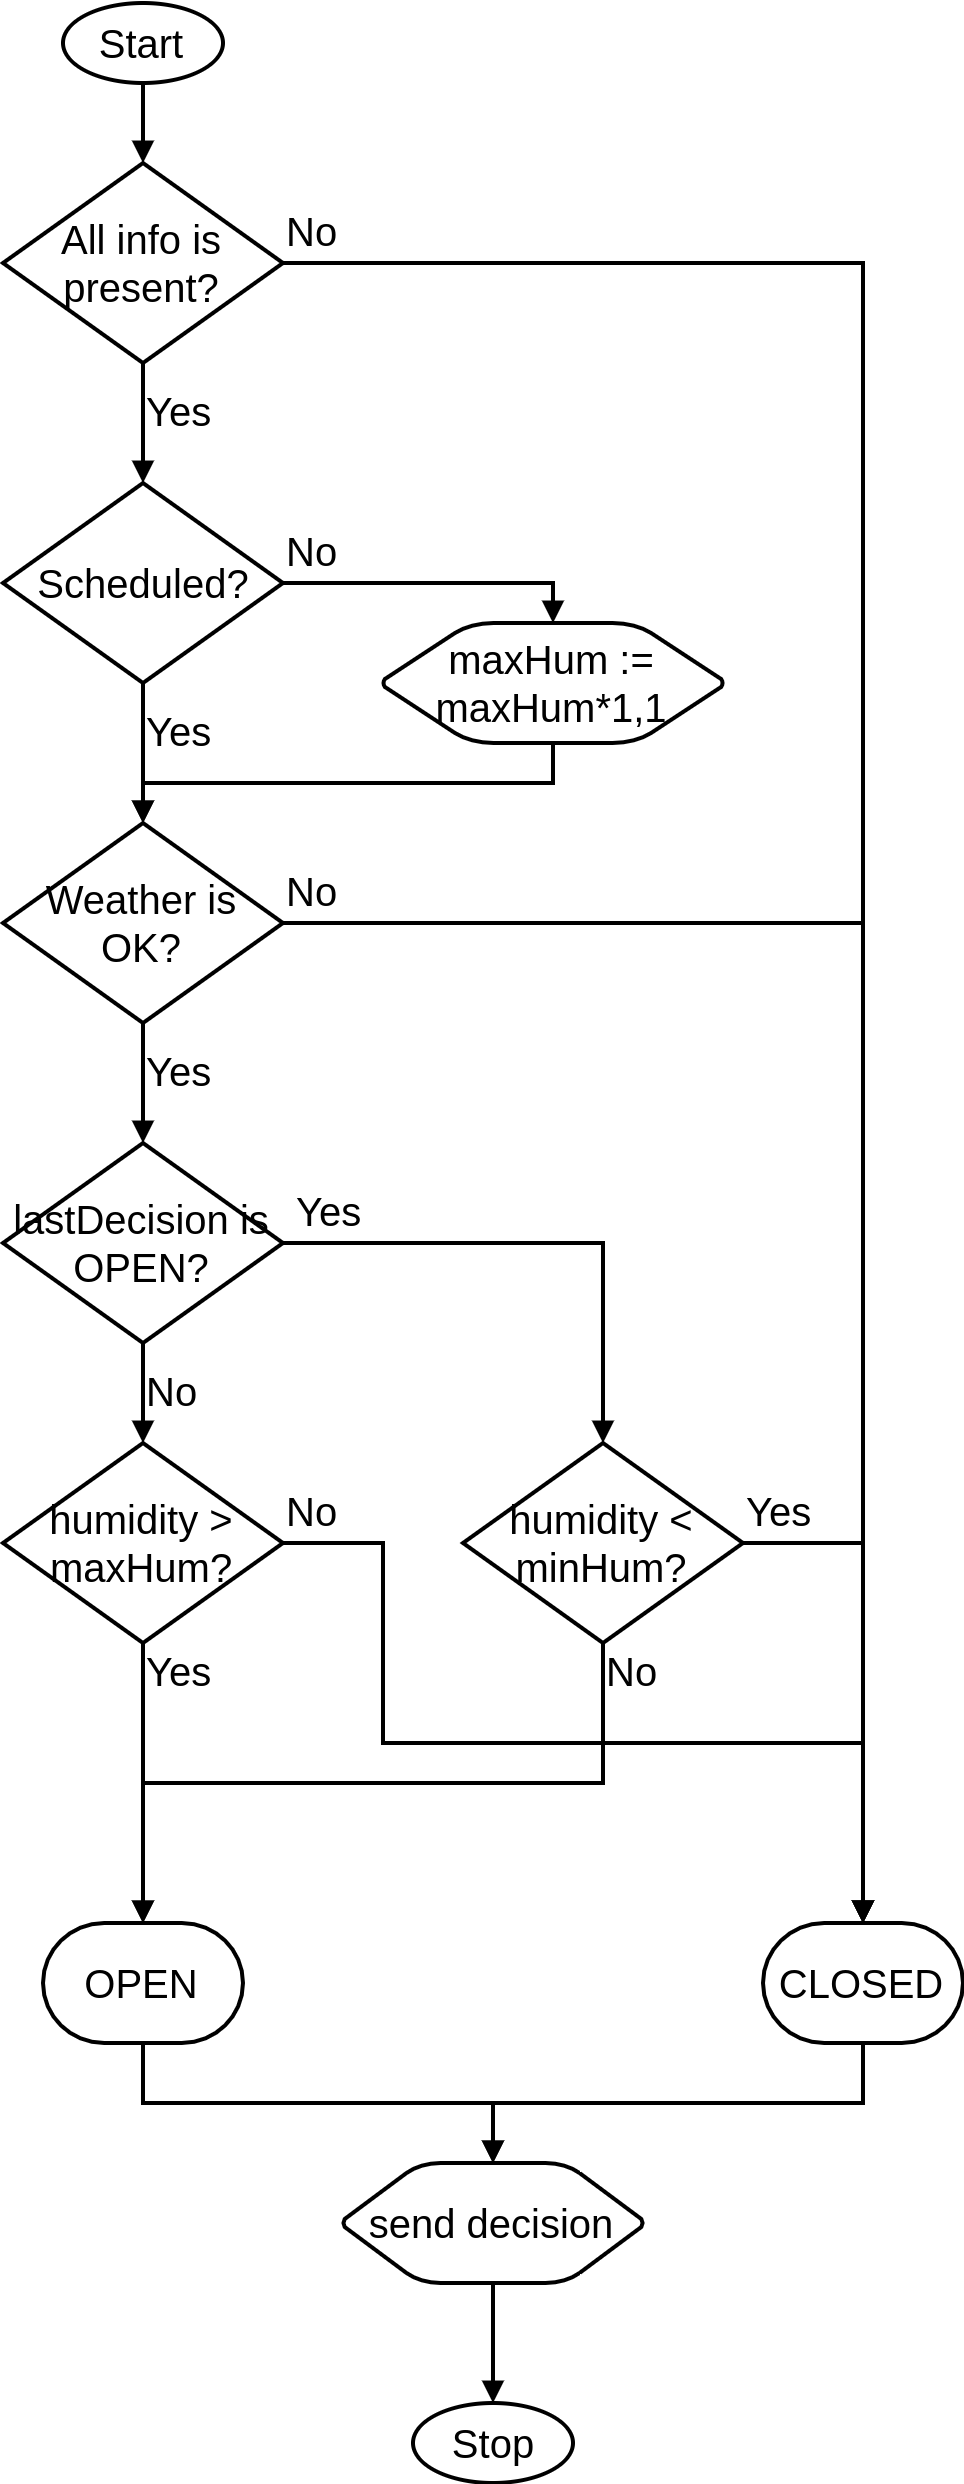
\includegraphics[width=250px]{imgs/decision_logic.png}
  \caption{Flow diagram of decision logic}
  \label{fig:decision_logic}
\end{figure} 

\section{Build tutorial}
\subsection{Prerequisites}

To build the application on Linux Mint 18.3 the following steps are needed:

\begin{itemize}
\item Install required packages with apt: 
\begin{itemize}
\item \verb+libboost-all-dev+
\item \verb+libcurl4-openssl-dev+
\item \verb+libssl-dev+ %(some help can be found \href{https://unix.stackexchange.com/a/389170}{here})
\item \verb+uuid-dev+
\item \verb+rapidjson-dev+
\item \verb+build-essential+
\item \verb+cmake+
\item \verb!g++!
\item \verb+git+
\end{itemize}
Use the following command:
\begin{lstlisting}
$ sudo apt install libboost-all-dev libcurl4-openssl-dev libssl-dev uuid-dev rapidjson-dev build-essential cmake g++ git
\end{lstlisting}
\item Install \href{http://www.curlpp.org/}{cURLpp} with the steps described \href{https://github.com/beniz/deepdetect/issues/126}{here}:
\begin{verbatim}
$ sudo apt-get remove libcurlpp0
$ mkdir curlppbuild
$ cd curlppbuild
$ git clone https://github.com/jpbarrette/curlpp.git
$ cd curlpp
$ cmake .
$ sudo make install
\end{verbatim} 
\item Install AzureIoT C SDKfrom \href{https://github.com/Azure/azure-iot-sdk-c/blob/master/doc/devbox_setup.md}{source}. After building the SDK use \verb+sudo make install+ to copy the header and the lib files to the system include path.
\item Download and install \href{https://www.rti.com/gettingstarted/installlinux_secure}{RTI Connext DDS 5.3}
\item Set the \verb+NDDSHOME+ environment variable to the root of RTI Connext DDS, e.g.: \verb+/opt/rti_connext_dds-5.3.0+
\end{itemize}
\begin{enumerate}

\subsection{Build process}
\item Clone git repository
\begin{lstlisting}
$ git clone https://github.com/antaljanosbenjamin/cps_homework.git
\end{lstlisting}
\item Generate source code from .idl files
\begin{lstlisting}[language=bash]
$ cd cps_homework
$ $NDDSHOME/bin/rtiddsgen  -language C++11 -stl -d DDS/Config/common -replace idl_files/Config.idl
$ $NDDSHOME/bin/rtiddsgen  -language C++11 -stl -d DDS/Decision/common -replace idl_files/Decision.idl
$ $NDDSHOME/bin/rtiddsgen  -language C++11 -stl -d DDS/Schedule/common -replace idl_files/Schedule.idl
$ $NDDSHOME/bin/rtiddsgen  -language C++11 -stl -d DDS/Humidity/common -replace idl_files/UvegHaz.idl
$ $NDDSHOME/bin/rtiddsgen  -language C++11 -stl -d DDS/Weather/common -replace idl_files/Weather.idl
\end{lstlisting}
\item Build
\begin{lstlisting}
$ mkdir build
$ cd build
$ cmake ..
$ make [-j 8]
\end{lstlisting}
\end{enumerate}

\section{Run demo}
\begin{enumerate}
\item Start humidity publisher
\begin{verbatim}
$ ./cps_main h <humidityDataFilePath>
\end{verbatim}

As result of this command the application will read the data file and start to publish a humidity value every 4 minutes. The file shall contains a humidity value per line. Each humidity value is a decimal number. See example \href{https://github.com/antaljanosbenjamin/cps_homework/blob/master/examples/humidity.txt}{file}.
\item Start IoTEdge 
\begin{lstlisting}
$ ./cps_main e <weatherApiKey> <azureConnectionString> <scheduleFilePath>
\end{lstlisting} 
The meaning of parameteres are the following:
\begin{itemize}
\item \verb+weatherApiKey+: an API key for http://api.airvisual.com
\item \verb+azureConnectionString+: the connection string of the device used Azure IoT Hub
\item \verb+scheduleFilePath+: path to a CSV file which stores the schedules time intervals. See example \href{https://github.com/antaljanosbenjamin/cps_homework/blob/master/examples/schedule.csv}{file}.
\end{itemize}
\item Start humidity controller
\begin{verbatim}
$ ./cps_main c
\end{verbatim}
\end{enumerate}

\end{document}
